% ********************************************
%
% BACKGROUND - BRIEF INTRODUCTION TO THE AREA
% OF RESEARCH CONCERNED AND CHALLENGE FACED
%
% ********************************************
\section*{Background}

In 1950, Alan Turing published a paper called 'Computing Machinery and Intelligence' \citep{turing-paper1950}, in which he posed the question, "Can machines think?". Alongside this question, he also proposed the Turing Test - a test that would use conversation to answer this question. Since then, Computer Scientists have been researching, for decades, how to develop chatterbots that converse convincingly with humans. Research, in this field, intensified when in the mid-1960s, Joseph Weizenbaum, developed ELIZA \citep{weizenbaum-eliza1966} - known to be the first chatter bot. ELIZA used an early-form of Natural Language Processing, where it would match patterns in the text input and substitute it with phrases, to create the illusion of understanding. In recent years, chatterbot developers have been trying to win the Loebner Prize - a modern day version of the Turing Test. This contest has been held since 1991 in which judges converse with chatterbots not knowing whether they are talking to a human or a chatterbot \citep{loebner-prize2001}. Chatterbots have also become very popular commercially, as businesses look to make their customer services more efficient, innovative and, most importantly, more personal, due to the rising demand of customers looking for fast resolutions to their problems and the increase in time they are spending online \citep{deloitte-chatbots2018}. This report by Deloitte, also found that one of the market forces driving chatterbot development is the "technological advances in AI and NLP".\\\\
Figure 1 below shows an infographic, also from the Deloitte report, displaying the "different functions of the human brain" that chatterbots try to "mimic". For my thesis, I will be concentrating on the Natural Language Processing (NLP) and Entity Recognition parts of the infographic for Dialog Management. NLP is a branch of AI concerned with the research of interactions between humans and computers through natural language. Natural Language has been defined in a white paper on NLP as being "the most natural means of communication between humans, and the mode of expression of choice for most of the documents they produce" \citep{nlp-whitepaper1989}. Entity Recognition (also known as Named Entity Recognition[NER]) is a branch of NLP concerned with labelling "sequences of words in a text which are the names of things, such as person and company names, or gene and protein names."  \citep{stanford-nlp-group}\\
\begin{figure}[h]
	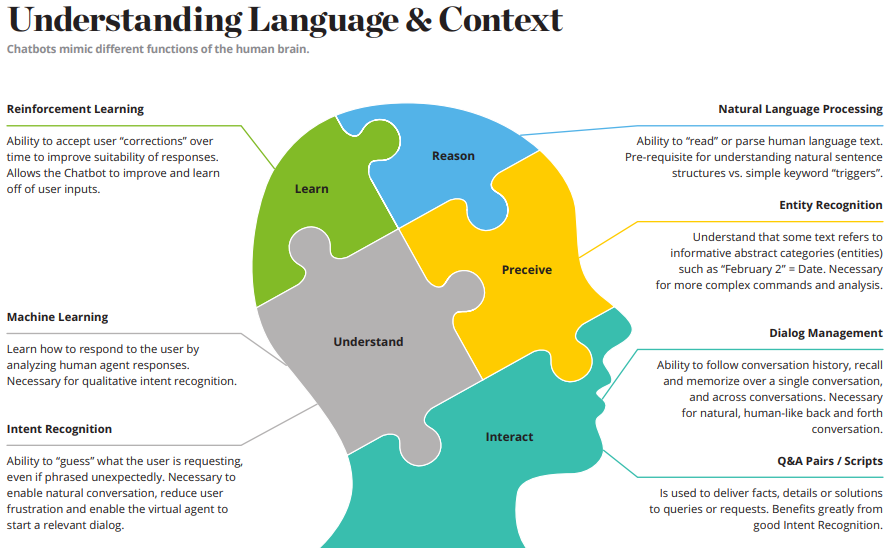
\includegraphics[width=\textwidth]{deloitte-infographic}
	\caption{Infographic showing the different functions of a chatterbot architecture \citep{deloitte-chatbots2018}}
\end{figure}\\
A big part of developing chatterbots is actually evaluating the quality of existing chatterbots and how convincing they are at mimicking the functions of the human brain. Two recent studies have tried to answer two questions that must be answered when evaluating the quality of a chatterbot. Firstly, the current uses of chatterbots in society must be examined. Brandtzaeg and Følstad have published their study of the uses of chatterbots on various platforms and across various categories of uses. \citep{why-people-use-chatbots2017} The vast majority of participants in the study reported using chatterbots to increase their productivity, by quickly retrieving information or accessing assistance. Rather surprisingly, the study also found that 12\% of the participants reported using chatterbots for social or relational use. The study found that the human nature of chatterbots drove people to using them for this purpose - the responses stated that chatterbots were a way of "avoiding loneliness" and "improving their social and conversational skills". Another study tried to gather together all the attributes and features that can be used to assess the quality of chatbots. \citep{evaluating-chatbots2017} The study found that two attributes that measures the effectiveness of the chatterbot are the ability to "maintain themed discussion" and to deliver "convincing, satisfying and natural interaction". The study also found that one of the attributes that measures the satisfaction of the chatterbot is the ability to "detect meaning or intent".\\\\
A big part of this project is to add a "long-term memory" mechanism to the core of the ELIZA chatterbot. Long-term memory is the ability to refer back to earlier conversations and to bring the information back at relevant points in the current conversation. This would make the chatterbot more human-like and, as discussed, would improve the quality of the chatterbot. I plan to achieve this using NER and NLP to store relevant and linked information into a database to retrieve at a later point in the conversation.
